% \iffalse meta-comment
%<*internal>
\def\nameofplainTeX{plain}
\ifx\fmtname\nameofplainTeX\else
\expandafter\begingroup
\fi
%</internal>
%
%
%
%
% ^^A -------------------------------------- .ins -------------------------------------
%<*install>
\input docstrip.tex
\keepsilent
\askforoverwritefalse
\preamble
----------------------------------------------------------------
utfpr-pg --- Classe para trabalhos acadêmicos da UTFPR-PG
Author:  Fabiano Rosas, Gabriel Casella
E-mail:  fabianorosas@gmail.com, gbc921@gmail.com
License: Released under the LaTeX Project Public License v1.3c or later
See:     http://www.latex-project.org/lppl.txt
----------------------------------------------------------------
\endpreamble

\postamble
Customizations of the abnTeX2 class (http://abnTeX2.googlecode.com)

This work may be distributed and/or modified under the
conditions of the LaTeX Project Public License (LPPL), either
version 1.3c of this license or (at your option) any later
version.  The latest version of this license is in the file:

http://www.latex-project.org/lppl.txt

This work is "maintained" (as per LPPL maintenance status) by
(not set).

This work consists of the file utfpr-pg.dtx and a Makefile.
Running make generates the derived files README.txt, utfpr-pg.pdf and utfpr-pg.cls.
Running make inst installs the files in the user's TeX tree.
Running make install installs the files in the local TeX tree.

Further information about abnTeX2 is available on http://abntex2.googlecode.com/
\endpostamble

\usedir{tex/latex/utfpr-pg}
\generate{
        \file{\jobname.cls}{\from{\jobname.dtx}{class}}
        \file{\jobname.bib}{\nopreamble\nopostamble\from{\jobname.dtx}{bibliography}}
}
%</install>
%<install>\endbatchfile
%<*internal>
\usedir{source/latex/utfpr-pg}
\generate{
        \file{\jobname.ins}{\from{\jobname.dtx}{install}}
}
\ifx\fmtname\nameofplainTeX
\expandafter\endbatchfile
\else
\expandafter\endgroup
\fi
%</internal>
% \fi
%
%
%
%
% ^^A---------------------------------------------- .dtx ----------------------------------------
% \iffalse
%<*driver>
\ProvidesFile{utfpr-pg.dtx}
%</driver>
%<class>\NeedsTeXFormat{LaTeX2e}[1999/12/01]
%<class>\ProvidesClass{utfpr-pg}
%<*class>
[2013/10/30 v1.00 Classe para trabalhos acadêmicos da UTFPR-PG]
%</class>
%<class>\DeclareOption*{\PassOptionsToClass{\CurrentOption}{abntex2}}
%<class>\ProcessOptions\relax
%<*driver>
\documentclass{ltxdoc}
\usepackage[a4paper,margin=25mm,left=50mm,nohead]{geometry}
\usepackage[numbered]{hypdoc}
\usepackage[utf8]{inputenc}
\usepackage[T1]{fontenc}
\usepackage{xcolor}
\usepackage{pbox}
\usepackage{url}
\usepackage{subcaption}
\usepackage{graphicx}
\usepackage[within=none]{newfloat}
\usepackage[font=itshape]{quoting}
\usepackage[brazil]{babel}
\usepackage[alf,abnt-emphasize=bf,abnt-repeated-author-omit=yes]{abntex2cite}
\usepackage{array}
\definecolor{dark-gray}{gray}{0.20}
\definecolor{light-gray}{gray}{0.85}

\newcommand\linha{\leavevmode\xleaders\hbox{-}\hfill\kern0pt}

\DeclareFloatingEnvironment[
fileext=loq,
listname=Lista de Quadros,
name=Quadro,
placement=tbhp,
]{quadro}

\EnableCrossrefs
%^^A\CodelineIndex
\begin{document}
\DocInput{\jobname.dtx}
\end{document}
%</driver>
% \fi
%
% \GetFileInfo{\jobname.dtx}
% \DoNotIndex{\newcommand,\newenvironment,\center}
%
% \title{\textsf{utfpr-pg} --- Classe para trabalhos acadêmicos da UTFPR-PG.}
%
% \author{Fabiano Rosas\\Gabriel Casella\thanks{fabianorosas@gmail.com, gbc921@gmail.com}}
% \date{Released \filedate}
%
% \maketitle
%
%
% \begin{abstract}
%   Com o intuito de aproveitar as facilidades introduzidas pela classe abn\TeX2 para a formatação de trabalhos acadêmicos de acordo com as normas da \textbf{ABNT} está sendo desenvolvida a classe \textsf{utfpr-pg}, que implementa as normas de formatação de trabalhos acadêmicos da Universidade Tecnológica Federal do Paraná, campus Ponta Grossa.
% \end{abstract}
%
%
%
% \section{As normas da UTFPR}
% A implementação das normas para trabalhos acadêmicos da UTFPR-PG está sendo feita tomando por base a classe abn\TeX2 \url{http://abntex2.googlecode.com/}.
%
% Como existem algumas diferenças com relação à norma atual da ABNT (implementada pela abn\TeX2) e as normas da UTFPR, esta classe tem o intuito de reproduzir da maneira mais fiel possível o que está documentado no manual ``Normas para elaboração de trabalhos acadêmicos'', presente em \url{http://www.utfpr.edu.br/dibib/normas-para-elaboracao-de-trabalhos-academicos/normas_trabalhos_utfpr.pdf}.
%
% Juntamente com o manual de normas, um documento-modelo (|.doc|) é comumente provido pela UTFPR. Este documento representa apenas uma das possíveis formas de formatação de um trabalho acadêmico recomendadas pela norma, portanto não iremos levá-lo em consideração para evitar conflitos.
%
%\iffalse
\LoadClass[a4paper]{abntex2}
\RequirePackage[alf,abnt-emphasize=bf,abnt-repeated-author-omit=yes]{abntex2cite}
\RequirePackage{indentfirst}
\RequirePackage[utf8]{inputenc}
\RequirePackage{lastpage}
\RequirePackage{etoolbox}
\RequirePackage{multibib}
\RequirePackage[within=none]{newfloat}
%\fi
%
%
%
% \section{Informações para o usuário}
% Nesta seção estão as intruções de uso para aqueles que desejam produzir trabalhos acadêmicos formatados nas normas da UTFPR.
% \subsection{Obtenção}
% \label{sec:obtencao}
%
% A obtenção da classe pode ser feita através do link: \url{https://github.com/UTFPR-PG/latex}.
%
%
%
% \subsection{Utilização}
% A utilização da classe é feita usando o nome da classe como argumento do comando |documentclass| da seguinte forma: |\documentclass{utfpr-pg}|. Os exemplos presentes no repositório podem servir como um ponto de partida.
%
%\iffalse ^^A inicia a classe, mas não mostra a tag no pdf
%<*class>
%\fi
%
%
%
% \subsection{Comandos pré-definidos (macros)}
% Além dos comandos padrão da abn\TeX2, como por exemplo, |\autor|, |\titulo| e |\local|, a classe da UTFPR define as seguintes macros:
%
% \DescribeMacro{\utfpr}
% Insere o texto ``Universidade Tecnológica Federal Do Paraná''.
%
% \DescribeMacro{\curso}
% Usa-se para definir o curso de graduação ou especialização.
%
% \DescribeMacro{\departamento}
% Usa-se para definir o departamento, coordenação ou programa.
%
%\iffalse
\newcommand\utfpr{Universidade Tecnológica Federal Do Paraná}
\newcommand*\erro[1]{\@latex@error{Defina \noexpand#1!}\@ehc}

\providecommand\imprimircurso{\erro\curso}
\newcommand*\curso[1]{\renewcommand{\imprimircurso}{#1}}

\providecommand\imprimirdepartamento{}
\newcommand*\departamento[1]{\renewcommand{\imprimirdepartamento}{#1}}
%\fi
%
%
%
% \subsection{Ambientes}
% \DescribeMacro{\listadequadros}
% A classe UTFPR-PG provê o ambiente \textsf{Quadro} e o comando |\listadequadros|
%
% Outros ambientes podem ser criados pelo usuário seguindo o seguinte modelo:
%    \begin{macrocode}
\DeclareFloatingEnvironment[
    fileext=loq,
    listname=Lista de Quadros,
    name=Quadro,
    placement=tbhp,
]{quadro}
%    \end{macrocode}
% A utilização dos novos ambientes é feita da mesma maneira que o ambiente \textsf{figure}, por exemplo:
%
% \begin{verbatim}
% \begin{quadro}
% \centering
%   \begin{tabular}{|l|l|l|l|l|}
%    \hline
%    Isto   & a & b & c & d\\ \hline
%    é      & a & b & c & d\\ \hline
%    um     & a & b & c & d\\ \hline
%    quadro & a & b & c & d\\ \hline
%  \end{tabular}
% \caption{Exemplo de quadro}
% \end{quadro}
% \end{verbatim}
% 
% Produz o seguinte quadro:
%
% \begin{quadro}
% \centering
%   \begin{tabular}{|l|l|l|l|l|}
%     \hline
%    Isto   & a & b & c & d\\ \hline
%    é      & a & b & c & d\\ \hline
%    um     & a & b & c & d\\ \hline
%    quadro & a & b & c & d\\ \hline
%  \end{tabular}
% \caption{Exemplo de quadro}
% \end{quadro}
%
%
%
% \subsection{Capa}
% Para exibir a capa, utiliza-se o comando |\imprimircapa|.
% \begin{macro}{\imprimircapa}
%   A macro |\imprimircapa| da classe abn\TeX2 imprime um modelo básico de capa que atende aos requisitos da seção 4.1.1 da ABNT NBR~14724:2011. A capa não é incluída no bookmark do PDF.
%
%   Esta macro foi redefinida para atender às necessidades da UTFPR-PG.
% \end{macro}
%
%
%
% \subsection{Folha de rosto}
% Para exibir a folha de rosto, utiliza-se o comando |\imprimirfolhaderosto|.
% \begin{macro}{\imprimirfolhaderosto}
%   A macro |\imprimirfolhaderosto| insere a folha de rosto no texto. A folha de rosto está de acordo com a norma da UTFPR. Embora o arquivo |.doc| provido pela biblioteca como exemplo das normas contenha o nome de autor, local e data em negrito, o manual de normas não exige tal formatação. A página 25 do manual exibe um exemplo de folha de rosto sem negrito nas referidas entradas.
% \end{macro}
%
%
% 
% \subsection{Fonte}
% A norma da ABNT não especifica um tipo de fonte a ser utilizado, porém as normas da UTFPR-PG sugerem que para o uso com \LaTeX\ seja utilizada a fonte Nimbus, que é uma fonte parecida com a Times New Roman. A fonte Times é de propriedade da Microsoft e o seu uso requer licença.
%
%
%
% \subsection{Espaçamentos}
% Existem alguns espaçamentos que podem variar e portanto provemos aqui alguns comandos para que o usuário os modifique:
%
% \DescribeMacro{parágrafo}
% Com relação à indentação inicial do parágrafo, é recomendado utilizar de 1,5 a 2,5 cm. O valor definido por padrão é 1,5 cm. Para modificar este valor, basta utilizar o comando |\setlength\parindent|\marg{tamanho} .
%
% \DescribeMacro{margens}
% Para modificar o tamanho das margens, pode-se utilizar os comandos a seguir:
%    \begin{macrocode}
 \setlrmarginsandblock{3cm}{2cm}{*}
 \setulmarginsandblock{3cm}{2cm}{*}
 \checkandfixthelayout
%    \end{macrocode}
%
% \DescribeMacro{títulos}
% O espaçamento entre os títulos e o texto que os precede e sucede pode ser alterado com |\setlength\afterchapskip|\marg{tamanho} e |\setlength\beforechapskip|\marg{tamanho}.
%
%
%
% \subsection{Resumo}
% Sobre o resumo, a norma diz:
% \begin{quoting}
%   O texto deverá conter no máximo 500 palavras e ser antecedido pela referência do estudo. Também, não deve conter citações. O resumo deve ser redigido em parágrafo único, espaçamento simples e seguido das palavras representativas do conteúdo do estudo, isto é, palavras-chave, em número de três a cinco, separadas entre si por ponto e finalizadas também por ponto.
% \end{quoting}
%
% Para incluir a referência do próprio estudo, será necessário que o usuário produza duas entradas \textit{bibtex} com os seus dados e nomeie as chaves destas entradas como |this| e |thisen|, para referência em português e inglês, respectivamente. Veja o exemplo abaixo:
%
% \begin{verbatim}
%@thesis{this,
%    author={Aluno, Nome do},
%    title = {{Titulo do trabalho de conclusão de curso}},
%    year={2014},
%    type={Trabalho de conclusão de curso}
%}
%
%@thesis{thisen,
%    author={Aluno, Nome do},
%    title = {{Thesis title}},
%    year={2014},
%    type={BSc. Thesis}
%}
%\end{verbatim}
%
% É importante observar que as entradas não precisam ser do tipo |@thesis|, basta apenas que contenham as chaves (this, thisen) corretas. Estas entradas devem ser colocadas no seu arquivo |.bib|, juntamente com as outras referências.
%
% \DescribeMacro{\refthis}
% Para exibir a referência antes do resumo e do \textit{abstract}, insira, como primeira linha do ambiente, o comando |\refthis|\oarg{en}\marg{bib file}, conforme o exemplo abaixo. Suponha um arquivo de referências chamado |referencias.bib|.
%
% \begin{verbatim}
%\begin{resumo}
%    \refthis{referencias}
%
%    Texto do resumo contendo no máximo 500 palavras.
%
%    \vspace{\onelineskip}
%    \noindent
%    \textbf{Palavras-chaves}: palavras. chaves.
%\end{resumo}
%
%\begin{resumo}[Abstract]
%    \begin{otherlanguage*}{english}
%    \refthis[en]{referencias}
%
%    Abstract text with a maximum word-count of 500.
%
%    \vspace{\onelineskip}
%    \noindent
%    \textbf{Key-words}: key. words.
%    \end{otherlanguage*}
%\end{resumo}
% \end{verbatim}
% 
% Será necessário compilar as duas entradas separadamente, da seguinte forma:
% 
%\begin{verbatim}
%pdflatex arquivo.tex
%bibtex arquivo.aux
%bibtex this.aux
%bibtex thisen.aux
%pdflatex arquivo.tex
%pdflatex arquivo.tex
%\end{verbatim}
% ^^A ------------------------------------- enduser -------------------------------------------
% \section{Informações para o desenvolvedor}
% Esta seção contém informações para aqueles que estão fazendo o desenvolvimento e manutenção da classe, bem como aqueles que por algum motivo específico precisam de mais detalhes sobre a implementação.
%
% \subsection{Capa}
% Um ponto onde há diferenças visíveis entre as normas da ABNT e as normas da UTFPR é a capa. O livreto de normas da UTFPR, cita que a capa é:
%
% \begin{quoting}
%   elemento obrigatório, proteção externa que reveste o trabalho. Na capa devem constar informações de identificação da obra:
%   \begin{itemize}
%   \item nome da Instituição e do Curso, completos;
%   \item nome do autor(es): responsável intelectual ou artístico do trabalho;
%   \item título principal do trabalho: claro, preciso, com palavras que identifiquem o seu conteúdo;
%   \item subtítulo (se houver): deve ser evidenciada a sua subordinação ao título principal, precedido de dois pontos (:);
%   \item número de volume (se houver mais de um deve constar, em cada capa, a especificação do respectivo volume);
%   \item tipo de documento científico ou acadêmico (tese, dissertação, trabalho de conclusão de curso, monografia de especialização, relatório de pesquisa, ou tros trabalhos acadêmicos);
%   \item local (cidade) da Instituição onde o trabalho deve ser apresentado;
%   \item ano de depósito (entrega do trabalho).
%   \end{itemize}
% \end{quoting}
%
% A capa foi definida da seguinte forma:
%\begin{macrocode}
\renewcommand{\imprimircapa}{
        \begin{capa}
          \center
          {\large\MakeUppercase\utfpr}\par
          {\large\MakeUppercase\imprimirdepartamento}\par
          {\large\MakeUppercase\imprimircurso}\par
          \vfill
          {\large\MakeUppercase\imprimirautor}\par
          \vfill
          {\bfseries\large\MakeUppercase\imprimirtitulo}\par
          \vfill
          {\large\MakeUppercase\imprimirtipotrabalho}\par
          \vfill
          {\large\MakeUppercase\imprimirlocal}\par
          {\large\imprimirdata}\par
        \end{capa}
}
%    \end{macrocode}
%
%
%
% \subsection{Folha de rosto}
% De acordo com as normas, a folha de rosto:
%
% \begin{quoting}
% É constituída de anverso e verso e tem os seguintes elementos:
% \begin{itemize}
% \item nome do autor (es): responsável intelectual ou artístico do trabalho;
% \item título principal do trabalho: claro, preciso, com palavras que identifiquem o seu conteúdo;
% \item subtítulo (se houver): deve ser evidenciada sua subordinação ao título principal, precedido de dois pontos (:);
% \item número de volumes (se houver mais de um, deve constar em cada folha de rosto a especificação do respectivo volume);
% \item tipo de documento científico ou acadêmico (tese, dissertação, trabalho de conclusão de curso e outros) e objetivo (aprovação em disciplina, grau pretendido e outros); nome da instituição a que será submetido, área de concentração;
% \item nome do orientador e do co-orientador (se houver);
% \item local (cidade) da instituição onde o trabalho deve ser apresentado;
% \item ano de depósito (da entrega).
% \end{itemize}
% \end{quoting}
%
% A folha de rosto foi definida da seguinte forma:
%    \begin{macrocode}
\renewcommand{\folhaderostocontent}{
  \begin{center}

    {\large\MakeUppercase\imprimirautor}
	
    \vspace*{\fill}\vspace*{\fill}
    \begin{center}
      {\bfseries\large\MakeUppercase\imprimirtitulo}\par
    \end{center}
    \vspace*{\fill}
	
    \abntex@ifnotempty{\imprimirpreambulo}{%
      \hspace{.45\textwidth}
      \begin{minipage}{.5\textwidth}
      	\SingleSpacing
         \imprimirpreambulo
       \end{minipage}%
       \vspace*{\fill}
    }%

    {\large\imprimirorientadorRotulo~\imprimirorientador\par}
    \abntex@ifnotempty{\imprimircoorientador}{%
       {\large\imprimircoorientadorRotulo~\imprimircoorientador}%
    }%
    \vspace*{\fill}

    {\large\MakeUppercase\imprimirlocal}\par
    \par
    {\large\imprimirdata}
    \vspace*{1cm}

  \end{center}
}
%    \end{macrocode}
%
% 
%
% \subsection{Fonte}
% A norma da ABNT não especifica um tipo de fonte a ser utilizado, porém as normas da UTFPR-PG sugerem que para o uso com \LaTeX\ seja utilizada a fonte Nimbus. O pacote \textit{Gyre Termes} implementa as fontes da família Nimbus Roman No 9 L.
%    \begin{macrocode}
\RequirePackage{tgtermes}
%    \end{macrocode}
%
% Para as legendas das ilustrações e tabelas, é necessário o tipo negrito e recomenda-se o uso de fonte tamanho 10.
% ^^A Também é utilizado como largura máxima da legenda a mesma da ilustração ou tabela.
%    \begin{macrocode}
\RequirePackage[font=small,font=bf,labelfont=bf]{caption}
%    \end{macrocode}
%
%\iffalse
\renewcommand{\ABNTEXchapterfont}{\bfseries}
\renewcommand{\ABNTEXchapterfontsize}{\normalsize}
\renewcommand{\ABNTEXsectionfont}{}
\renewcommand{\ABNTEXsectionfontsize}{\normalsize}
%^^A\newcommand{\primeirasmaiusculas}[1]{\titlecap{#1}}
%^^A\setsubsecheadstyle{\primeirasmaiusculas}
\renewcommand{\ABNTEXsubsectionfontsize}{\normalsize}
\renewcommand{\ABNTEXsubsubsubsectionfont}{\itshape}
%\fi
%
%
%
% \subsection{Espaçamentos}
% A questão do espaçamento é bastante nebulosa, já que as medidas são todas especificadas sem unidades, ou em unidades imaginárias relacionadas ao MS Word. Um exemplo é o espaçamento entre-linhas que é definido como $1,5$. Teoricamente, o espaçamento entre-linhas é dado pelo |\baselineskip| de determinada fonte, que é a distância entre as bases de duas linhas de texto. O problema é que não há como saber se $1,5$ significa $1,5$ vezes o baseline ou um baseline de razão $1,5$ em relação ao tamanho da fonte. No \LaTeX, existem duas formas de se tratar isso:
%
% \begin{enumerate}
% \item Através do comando |\linespread| que multiplica o |\baselineskip|;
% \item Através do pacote |setspace| que altera o espaçamento levando em consideração o tamanho da fonte.
% \end{enumerate}
%
% Usar |\linespace| com valores $1.0$, $1.5$ e $2.0$ gera os espaçamentos simples, 1,5 e duplo, de maneira muito semelhante ao MS Word. Já o pacote |setspace|, cria espaçamentos menores, como se usássemos |\linespace{1.3}| ao invés de |\linespace{1.5}| para espaçamento 1,5.
%
% Nesta classe, usaremos o padrão implementado pelo |memoir.cls|, que é igual ao |setspace| devido ao fato de ser o mais recomendado pela comunidade e por que o comando |\linespread| altera a formatação de tabelas e notas de rodapé de maneira indesejável. A implementação do |memoir.cls| é feita através dos comandos |\SingleSpacing|, |\OnehalfSpacing| e |\DoubleSpacing|.
%
% Na seção 3.3 do manual de normas da UTFPR está previsto que:
% \begin{quoting}
% Nos elementos pré-textuais: o resumo, as notas, as referências, as legendas das ilustrações e tabelas, a ficha catalográfica, a natureza do trabalho, o objetivo, o nome da instituição a que é submetida e a área de concentração devem ser digitados em espaço simples;
% \end{quoting}
% Para isso, adicionamos um \textit{hook} ao comando |\pretextual|, aplicando o comando |\SingleSpacing|:
%
%    \begin{macrocode}
\pretocmd{\pretextual}{%
        \SingleSpacing}{}{%
        \ClassWarning{utfpr-pg}{%
                Erro ao modificar o comando \@backslashchar pretextual,
                isto pode ter causado algum erro de formatação no seu documento.
                Consulte os desenvolvedores da classe.}}
%    \end{macrocode}
%
% A norma prossegue, dizendo:
%
% \begin{quoting}
%   \begin{itemize}
%   \item no texto: todo o texto deve ser formatado com espaço 1,5 entre linhas;
%   \end{itemize}
% \end{quoting}
%
% De maneira análoga à anterior:
%    \begin{macrocode}
\pretocmd{\textual}{%
        \pagestyle{simple}%
        \OnehalfSpacing}{}{%
        \ClassWarning{utfpr-pg}{%
                Erro ao modificar o comando \@backslashchar textual,
                isto pode ter causado algum erro de formatação no seu documento.
                Consulte os desenvolvedores da classe.}}
%    \end{macrocode}
%
% A norma diz ainda:
%
% \begin{quoting}
%   \begin{itemize}
%^^A TODO:   \item nas citações: as citações com mais de três linhas devem ser em espaço simples;
%^^A TODO:  \item nas referências: as referências, ao final do trabalho, devem ser separadas entre si por dois espaços simples, e na mesma referência o espaço é simples;
%   \item nos títulos: os títulos das seções primárias e das demais subseções devem ser separados do texto que os precede ou que os sucede por dois espaços 1,5;
%   \end{itemize}
% \end{quoting}
% 
% Novamente não há como saber o que ``1,5'' significa. Usaremos um valor padrão e informaremos ao usuário como mudar este espaçamento caso necessário.
%
%    \begin{macrocode}
\setlength\beforechapskip{2.0\onelineskip}
\setlength\afterchapskip{2.0\onelineskip}

\setlength\beforesecskip{\beforechapskip}
\setlength\aftersecskip{\afterchapskip}

\setlength\beforesubsecskip{\beforechapskip}
\setlength\aftersubsecskip{\afterchapskip}

\setlength\beforesubsubsecskip{\beforechapskip}
\setlength\aftersubsubsecskip{\afterchapskip}
%    \end{macrocode}
%
% \begin{quoting}
%   \begin{itemize}
%   \item as seções primárias devem iniciar em páginas distintas.
%   \end{itemize}
% \end{quoting}
%
% Isto já está implementado pelo abn\TeX2.\\
%
%
% Com relação à indentação inicial do parágrafo, é recomendado utilizar de 1,5 a 2,5 cm. O valor definido por padrão é 1,5 cm:
%
%    \begin{macrocode}
\setlength\parindent{1.5cm}  
%    \end{macrocode}
%
%
%
% \subsection{Sumário}
% As modificações feitas para acomodar as normas referentes ao sumário estão listadas a seguir.
%
% \subsubsection{Espaçamento}\label{s:esp}
% As entradas do sumário estão sendo ajustadas de maneira dinâmica para evitar o problema que ocorre quando a numeração de uma seção fica muito grande e sobrepõe o texto. Na figura \ref{f:sumariotruncado}, o espaçamento entre o número do capítulo e a palavra ``capítulo'' está correto, porém, conforme as seções vão ramificando ou os números aumentando, a visualização vai ficando truncada. O comportamento correto é o apresentado na figura \ref{f:sumariocorreto}.
% \begin{figure}[h]
%   \centering
%   \begin{subfigure}[b]{0.4\textwidth}
%     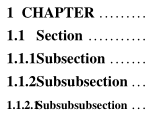
\includegraphics[scale=.95]{imagens/sumariotruncado.png}
%     \caption{Incorreto}
%     \label{f:sumariotruncado}
%   \end{subfigure}
%   \begin{subfigure}[b]{0.4\textwidth}
%     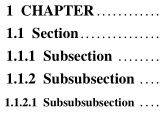
\includegraphics{imagens/sumariocorreto.png}
%     \caption{Correto}
%     \label{f:sumariocorreto}
%   \end{subfigure}
%   \caption{Apresentação do sumário}
% \end{figure}
%
% O ajuste das entradas foi feito alterando a macro |\numberlinehook| que é expandida dentro da macro responsável por exibir o número da seção (1.1, 1.2.1, etc\ldots) de forma que o tamanho da caixa onde fica o número seja ajustado de acordo com o espaço que o número ocupa:
%
%    \begin{macrocode}
\renewcommand\numberlinehook[1]{%
        \addtolength{\@tempdima}{\widthof{#1}}
}
\renewcommand\chapternumberlinehook\numberlinehook
%    \end{macrocode}
%
% além disso, é necessário zerar a identação das entradas:
%
%    \begin{macrocode}
\renewcommand{\tocprintchapter}{
       \addtocontents{toc}{\cftsetindents{chapter}{0em}{1em}}}
\cftsetindents{chapter}{0em}{1em} % here for backwards compatibility, the corret way is the above
\cftsetindents{section}{0em}{1em}
\cftsetindents{subsection}{0em}{1em}
\cftsetindents{subsubsection}{0em}{1em}
%    \end{macrocode}
%
% O espaço antes dos capítulos também é eliminado:
%
%    \begin{macrocode}
\setlength\cftbeforechapterskip{0cm}
%    \end{macrocode}
%
%
%
% \subsubsection{Formatação}
% A formatação das entradas do sumário deve ser feita seguindo a imagem \ref{f:sumario}, ignorando-se as discrepâncias com relação ao espaçamento, que já foram corrigidas na seção \ref{s:esp}.
%\begin{figure}[h]
%  \centering
%  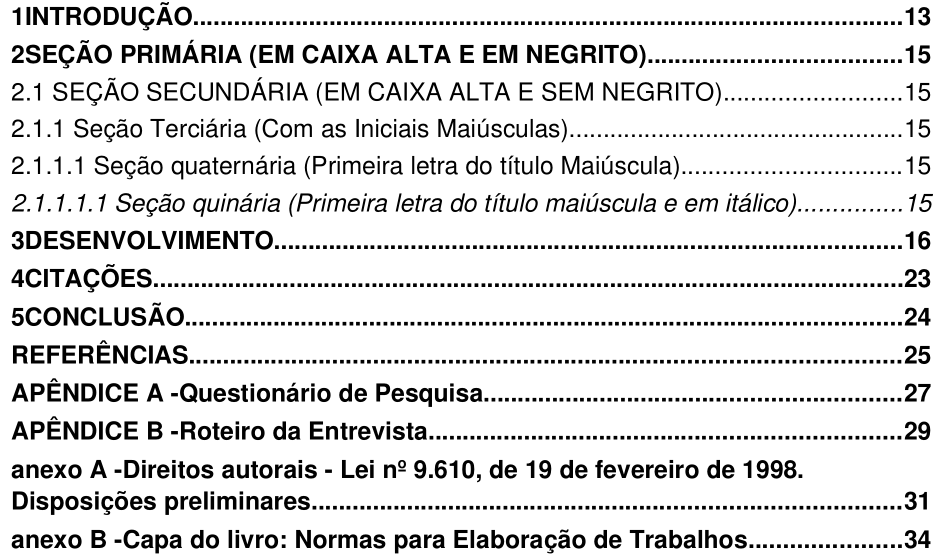
\includegraphics[scale=.3]{imagens/sumario.png}
%  \caption{Sumário de acordo com o livreto de normas da UTFPR}
%  \label{f:sumario}
%\end{figure}
%
% Algumas das modificações necessárias já foram feitas quando se modificaram as fontes para os capítulos, seções, etc., restando aqui as que são relativas ao sumário apenas:
%
%^^A \renewcommand{\cftchapterfont}{\bfseries} já está na seção Fonte
%    \begin{macrocode}
\renewcommand{\cftchapterleader}{\normalfont\cftdotfill{\cftchapterdotsep}}
\renewcommand{\cftchapterpagefont}{\normalfont}
\renewcommand{\cftdotsep}{1}
%    \end{macrocode}
%^^A\newcommand{\upcase}[1]{\uppercase{#1}} mover p/ seção Fonte
%^^A\renewcommand{\cftsectionfont}{\mdseries\upcase} mover p/ seção Fonte
%^^A\renewcommand{\cftsubsectionfont}{\mdseries} mover p/ seção Fonte
%^^A\renewcommand{\cftsubsubsectionfont}{\mdseries} mover p/ seção Fonte
% 
% As referências devem aparecer como um capítulo normal no sumário:
%
%    \begin{macrocode}
\renewcommand{\bibsection}{\chapter*{\bibname}\prebibhook}
%    \end{macrocode}
%
%
%
% \subsection{Resumo}
% Sobre o resumo, a norma diz:
% \begin{quoting}
%   O texto deverá conter no máximo 500 palavras e ser antecedido pela referência do estudo. Também, não deve conter citações. O resumo deve ser redigido em parágrafo único, espaçamento simples e seguido das palavras representativas do conteúdo do estudo, isto é, palavras-chave, em número de três a cinco, separadas entre si por ponto e finalizadas também por ponto.
% \end{quoting}
%
% Para incluir a referência do próprio estudo, utilizaremos o pacote |multibib| para inserir duas bibliografias, uma que funcionará normalmente e será apresentada no final do trabalho e outra que servirá apenas para referenciarmos o próprio trabalho. Esta bibliografia será exibida antes do resumo. Apesar de haver duas bibliografias, o arquivo |.bib| que contém as entradas é um só \footnote{Apesar disso, é preciso rodar o |bibtex| nos dois |.aux| extra que serão gerados.}.
%
% Será necessário que o usuário produza duas entradas \textit{bibtex} com os seus dados e nomeie as chaves destas entradas como |this| e |thisen|, para referência em português e inglês, respectivamente.\\
%
% O processo funciona da seguinte forma.\\
% 
% Definimos duas novas bibliografias com um texto vazio:
%    \begin{macrocode}
\newcites{this}{ }
\newcites{thisen}{ }
%    \end{macrocode}
%
% Definimos um comando que recebe como parâmetro o nome da bibliografia a ser utilizada:
%    \begin{macrocode}
\newcommand\refthis[2][]{
\begingroup
\let\clearpage\relax
\vspace{-40pt}
\expandafter\csname nocitethis#1\endcsname{this#1}
\expandafter\csname bibliographystylethis#1\endcsname{abntex2-\AbntCitetype}
\expandafter\csname bibliographythis#1\endcsname{#2}
\vspace{\onelineskip}
\endgroup
}
%    \end{macrocode}
%
% Agora basta que o usuário inclua o comando |\refthis|\oarg{en}\marg{bib file} antes do texto do resumo ou \textit{abstract}.
%
%
%
%\iffalse ^^A finaliza a tag classe, mas nao mostra no pdf
%</class>
%\fi
%\iffalse ^^A evita que o conteudo do .bib apareça no pdf
% ^^A -------------------------------------- .bib -------------------------------------
%<*bibliography>
@misc{nimbus,
        title = {Nimbus Roman},
        author = {The {LaTeX} Font Catalogue},
        url = {http://www.tug.dk/FontCatalogue/nimbus/},
        urldate = {2013-11-01},
        year = {2013},
        file = {The LaTeX Font Catalogue – Nimbus Roman:/home/fabiano/.zotero/zotero/ru3nfjod.default/zotero/storage/2I5F789D/nimbus.html:text/html}
},

@misc{gyre,
        title = {{TeX} Gyre Termes},
        author = {The {LaTeX} Font Catalogue – },
        url = {http://www.tug.dk/FontCatalogue/tgtermes/},
        urldate = {2013-11-01},
        year = {2013},
        file = {The LaTeX Font Catalogue – TeX Gyre Termes:/home/fabiano/.zotero/zotero/ru3nfjod.default/zotero/storage/FAVQWTBI/tgtermes.html:text/html}
}

@misc{abntex2,
        title = {A classe abntex2: Documentos técnicos e científicos brasileiros compatíveis com as normas ABNT},
        author = {Lauro César Araújo},
        url = {http://ctan.tche.br/macros/latex/contrib/abntex2/doc/abntex2.pdf},
        year = {2014}
}

@manual{memoir,
  title = {The Memoir Class},
  author = {Peter Wilson},
  month = {Abril},
  year = {2013},
  owner = {fabiano},
  timestamp = {2014.02.24},
  url = {http://repositorios.cpai.unb.br/ctan/macros/latex/contrib/memoir/memman.pdf}
}

@manual{latex2e,
  title = {LaTeX2e for class and package writers},
  organization = {The LaTeX 3 Project},
  month = {Março},
  year = {1999},
  owner = {fabiano},
  timestamp = {2014.02.24},
  url = {http://latex-project.org/guides/clsguide.pdf}
}

@manual{package,
  title = {How to package your LaTeX package},
  author = {Scott Pakin},
  month = {Novembro},
  year = {2004},
  owner = {fabiano},
  timestamp = {2014.02.24},
  url = {http://www.tex.ac.uk/ctan/info/dtxtut/dtxtut.pdf}
}

@manual{abntex2cite,
  title = {O pacote abntex2cite: Estilos bibliográficos compatíveis com a ABNT NBR 6023},
  author = {Lauro César Araújo},
  month = {Janeiro},
  year = {2014},
  owner = {fabiano},
  timestamp = {2014.02.24},
  url = {http://repositorios.cpai.unb.br/ctan/macros/latex/contrib/abntex2/doc/abntex2cite.pdf}
}

%</bibliography>
%\fi
%
%
% \nocite{abntex2cite}
% \nocite{package}
% \nocite{latex2e}
% \nocite{memoir}
% \nocite{abntex2}
% \nocite{gyre}
% \nocite{nimbus}
% \bibliography{utfpr-pg}
%
%
\endinput
% \Finale
